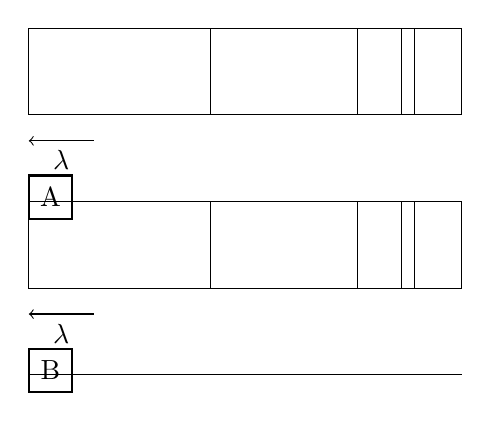
\begin{tikzpicture}[x=0.55cm,y=0.55cm]
% Row 1: unlabeled wave train
\draw (0,10) rectangle (10,12);
\draw (4.2,10) -- (4.2,12);
\draw (7.6,10) -- (7.6,12);
\draw (8.6,10) -- (8.6,12);
\draw (8.9,10) -- (8.9,12);
\draw[->] (1.5,9.4) -- (0,9.4) node[midway,below] {$\lambda$};
% Row 2: labeled A
\draw (0,6) rectangle (10,8);
\draw[thick] (0,7.6) rectangle (1,8.6);
\node at (0.5,8.1) {A};
\draw (4.2,6) -- (4.2,8);
\draw (7.6,6) -- (7.6,8);
\draw (8.6,6) -- (8.6,8);
\draw (8.9,6) -- (8.9,8);
\draw[->] (1.5,5.4) -- (0,5.4) node[midway,below] {$\lambda$};
% Row 3: labeled B (cropped, only top edge visible)
\draw (0,4) -- (10,4);
\draw[thick] (0,3.6) rectangle (1,4.6);
\node at (0.5,4.1) {B};
\end{tikzpicture}
